\chapter{Introduction}
\thispagestyle{empty}

For over a century, the scientific community has invested efforts into developing energetic particle and X-ray sources. This research was driven by the need to study matter on the atomic scale, or even below, with the investigation of elementary particle behavior. The fluence, duration, or spectral emission range of these sources have to be controlled to guarantee the success of an experiment. A particle beam can be composed of simple atoms or molecules (neutrals) or most commonly electrons or ions. On the scale of a nucleus, we can also find products of nuclear reactions (protons, neutrons) and fundamental particles (quarks, leptons..) as studied at CERN. The study of nuclear and fundamental reactions goes beyond the scope of this work because it requires large-scale accelerators ($\sim$TeV energies), unaccessible to an average laser facility. At the Laboratoire d'Optique Appliquée (LOA), our efforts are directed towards the comprehension and development of laser-driven generators of electromagnetic sources (X-UV\footnote{Extreme Ultraviolet: wavelengths between $10$ and $130\,\mathrm{nm}$} in our case) and  particle accelerators (electrons in our case) through laser-plasma interaction schemes. \\


\section{Why do we study plasmas ?}

A plasma is a state of matter where atoms are dissociated into electrons and positively charged ions either completely or partially. Although natural plasmas are rarely encountered on Earth, it is however the most abundant state in the universe and represents 99.9\% of visible state of matter. Therefore, the study of plasmas allows a better comprehension of our universe.  A plasma is characterized by various parameters among which its electron density and its temperature, provided it has reached thermal equilibrium. A common property of plasmas is their ability to emit electromagnetic and/or particle radiations. This is why astrophysical plasmas can be observed from the Earth. The spectral content of this emission is strongly related to their thermodynamical properties and chemical constituents. For instance, interstellar regions are  low-density plasmas  with less than $1\,\mathrm{electron/cm^3}$ and temperatures between $0.1$ and $100\,\mathrm{eV}$. Most of the spectral emission is in the far infrared. Dense plasmas ($\sim 10^{20-25}\,\mathrm{electron/cm^3}$) are encountered in the core of stars like the Sun, where strong thermonuclear reactions prevent the whole structure from collapsing under its own weight. Stars are classified according to their emission spectra going from infrared (cold stars) to gamma rays (hot and turbulent stars). In addition, very intense particle jets (electrons, protons, nuclear reaction products) coming from stars are directly or indirectly observed to describe the core plasma dynamics on various geological time scales. To generate energetic electromagnetic and particle  radiation in a laboratory, we use lasers to create plasmas with micrometer-sized volumes and with densities and temperatures approaching those found in the core of stars. The lifetime of these plasmas is on the order of $10^{-8}$ second.


%(add zeta puppis in following picture)
\begin{figure}[H]
\begin{center}
\noindent\makebox[\textwidth]{
\includegraphics[width =0.9\textwidth]{../introduction/images/plasmaDiagrams.pdf}}\\
\caption{\label{fig:plasmaDiagrams} Examples of plamas sorted by density and temperature}
\end{center}
\end{figure}

\noindent In the attempt to recreate astrophysical plasmas in a laboratory, we have progressively realized that in addition to understanding better the nature of the radiation coming from space, we are also paving the way towards table-top energetic radiation with countless applications (imaging, spectroscopy, medical therapy, nuclear physics...). Over a century, the scientific community has gone from the study of the universe over geological time scale to the study of micrometric systems over proportionally short time scales.

\section{ Laser-plasma physics: historical context}

Before the 50's, the geophysical and astrophysical community essentially studied plasmas doing spectroscopy of partially ionized gas through electric discharges. 
 Langmuir and Tonks were the first to conduct a parametric investigation of partially ionized mercury in the 1920's~\cite{langmuir1923positive,TonksAndLangmuire}, attractive because of its low ionization potential. But in 1960, the first ruby laser would quickly open the door to laser-driven plasma physics. The first efforts were directed towards the creation of high-density plasmas in order to provoke nuclear fusion reactions. However, controlling fusion reactions was not a new idea in the 60's. Between 1936 and 1939, Atkinson, Bethe and Houtermans~\cite{atkinson,bethe1937nuclear,bethe1939energy} had come up with a classification of light elements eligible for fusion to explain the reactions in the core of stars. With no surprise, these scientists were also part of the Manhattan project in the 1940's. In the 1950's, studies on the control of nuclear reactions using magnetically confined plasmas lead to the conception of reactors called Tokamaks~\cite{artsimovich1945radiation,akhiezer1949interaction,rax2011physique}. Finally, Dawson explained in 1964\cite{dawson1964production} how a short ($\sim \,\mathrm{ns}$)\footnote{$1\,\mathrm{ns} = 10^{-9}\mathrm{s}$} intense ($\sim \,\mathrm{TW}$)\footnote{$1\,\mathrm{TW} = 10^{12}\,\mathrm{W}$, power provided by $\sim 500$ nuclear plants} laser pulse \cite{basov1964conditions,daiber1966laser} was an eligible candidate to initiate thermonuclear reactions inside a solid pellet target. These intensities and durations were precisely accessible to state-of-the-art lasers in the 70's\cite{brueckner1974laser}.
In 1974, the Lawrence Livermore National Laboratory (LLNL) conducted the first experiment part of the ``inertial confinement fusion program'' to demonstrate Deuterium/Tritium ignition, using a 20J,$\sim 10\,\mathrm{ns}$ Nd: glass, 1.06 micron laser. After decades of experimental investigation, it appeared that carefully shaping the laser pulse would reduce the energy necessary to trigger nuclear reactions . More insight into the different times scales involved in the plasma dynamics, from nanosecond to femtosecond (and most recently attosecond) has been gained. \\


\subsection{Plasmas: different time scales}

In Physics, the same system can be studied on different time scales. For instance, one uses thermodynamics to predict the final state of a gas. However, on a time scale much shorter than the collision time between two atoms, one should turn to classical kinematics instead. This is of course also true in plasma physics, where the adequate set of equations used to describe the motion of both ion and electron populations inside the plasma will be radically different depending on the time scale of the interaction. Thermonuclear plasmas inside Tokamaks, for instance, are confined during several seconds. Diffusion, convection  and turbulences occur on time scales varying between $\sim~\mathrm{ns}$ to $<1\mathrm{s}$~\cite{rax2011physique}. Rayleigh instabilities~\cite{rayleigh1878instability} grow by $\sim 1\mathrm{\mu m}$ in $\sim 1 \mathrm{ns}$~\cite{emery1982rayleigh} at the surface of laser-compressed pellets and prevent the ignition of fusion reactions~\cite{betti1998growth}. Note that in the latter example, $1\mathrm{\mu m} / 1\mathrm{ns} = 1\,\mathrm{nm/ps}$, which is the sound velocity inside plasmas~\cite{Kruer1988}. Therefore a fluid model is well suited to describe the plasma on a ns time scale over several microns, or on the picosecond time scale over several nanometers. However, using a fluid approach to predict the plasma evolution during one femtosecond over one picometer no longer makes sense. In this case, we reach the dimension of an atom and the time scale of electron collisions in a dense plasma: collisions can be neglected and the physics is now described by the equation of motion of a single electron. The study of plasmas on femtosecond time scales requires the use of femtosecond laser pulses, and a control of the plasma conditions with nanometer resolution. %Therefore, it becomes clear that improving the temporal resolution of a light source isn't enough if no effort is made to simultaneously increase the spatial resolution of the enagaged process observation


\subsection{Lasers: different time scales}

The comprehension of plasma dynamics is strongly related to the rapid evolution of  laser technologies. The temporal duration\footnote{The temporal duration of a laser pulse is defined by the Full Width of Half Maximum (FWHM) of the pulse in power. For a Gaussian pulse, this power is $\propto \exp(\frac{-4 \ln (2)t^2}{\tau_{fwhm}^2})$} of the laser pulse available from continuous (milliseconds) to ultrashort (femtoseconds) depends on the spectral bandwidth and the phase relation between each spectral component. This is  directly influenced by the properties (losses, dimension) of the laser cavity. The temporal duration of a laser, and simultaneously its maximum  peak power\footnote{Peak power for a pulse of energy $E_0$ and temporal duration $P$ $\approx E_0/\tau_{fwhm}$} can be boosted by two techniques, namely Q-switching and mode-locking.\\

\begin{itemize}
\item[$\bullet$]\g{1960: Q-switching:} By a temporal modulation of the losses, the lasing cavity is successively turned on or off. Many round trips occur in the cavity such that the final energy contained in the pulse exceeds by orders of magnitude that of continuous wave operation.\\
\item[$\bullet$]\g{1960-1970: Laser mode-locking:} Used in the generation of ultrashort ($\sim \mathrm{fs}$ to a few ps) pulses. The gain medium inside the cavity has a large bandwith and all the amplified frequencies superimpose coherently inside the cavity. As a result, they interfere constructively, and the cavity generates a continuous train of very short pulses.
\end{itemize}

\vspace{0.3in}

\noindent In Table~\ref{tab:laserPerfs}, we provide an incomplete list of laser systems with different temporal durations. When energetic pulses are required for a given application, the pulse will in general undergo chirped-pulse amplification (CPA)~\cite{maine1988generation}. However, the word record in laser power today which simultaneously combines (i) an ultrashort (6fs) pulse duration and (ii) a very energetic pulse($\sim 100\,\mathrm{mJ}$)~\cite{mikhailova2011ultra} is based on OPCPA~\cite{dubietis1992powerful}.\\

\begin{table}[H]
\begin{center}
\begin{tabular}{ccc}\toprule
Technology & year & temporal duration \\
\hline
Ruby & 1960 & $\sim \mathrm{ms}$ \\
Nd:YAG & 1964 & $\sim200 \mathrm{\mu s}$ \\
Nd:YAG - Q-switched & 1965 & < 1ns\\
Nd:YAG - mode locked& 1968& $\sim30 \mathrm{ps}$ \\
Nd:YLF- Q-switched & 1992& $\sim100\,\mathrm{ns}$ \\
Nd:YLF- mode locked & 1992& $\sim10 \mathrm{ps}$ \\
He-Ne & 1960 & continuous \\
$\mathrm{CO}_2$ & 1964 & $1-100 \mathrm{ns}$ \\
$\mathrm{CO}_2 $- Q-switched & 1964 & <1ns \\
Ti:sapphire & 1982& $\sim 500$ns \\
Ti:sapphire - mode locked& 1989& <10fs \\
\hline
\end{tabular}
\caption{\label{tab:laserPerfs} Example of different laser performances}
\end{center}
\end{table}



\noindent Q-switched lasers are today widely used for industrial applications involving laser processing of metal and medical applications. However, the first experiments on the generation of coherent X-UV light from plasmas were performed using nanosecond $\mathrm{CO}_2$~\cite{burnett1977harmonic,Carman1981} in the 80's. Those results where attributed to the formation of plasma mirrors and reproduced with shorter and more intense  laser pulses in recent years~\cite{Tarasevitch2000,monot2004high,TheseCedric,borot2011high}.


\section{Plasma mirrors}

\subsection{What is a plasma mirror ?}

A plasma mirror (PM) is by definition a plasma, which is highly reflective for electromagnetic radiation, depending of its spectral content. The lower the laser wavelength $\lambda$, the higher the plasma density $n_e$ needs to be. This is illustrated in Fig~\ref{fig:citicaldensitiy}, where we plot the plasma critical density\footnote{Density at which radiation of wavelength $\lambda$ is reflected by the plasma} $n_c [\mathrm{cm^{-3}}] = (1.1\times 10^{21})/(\lambda[\,\mathrm{\mu m}])^2$ as a function of laser wavelength. To be reflective, just like a mirror, the plasma needs an optical surface quality, which means the surface depth fluctuations should remain $<\lambda$. There are however two fundamental differences between a PM and a standard metallic mirror: the first is the "switchability" of the PM. Because most  materials submitted to a very intense electric field ($\gtrsim 10^{13}\,\mathrm{W/cm^2}$) will ionize on a very short time scale ($\sim fs$), most materials can be "switched" into a mirror, during a time corresponding to the PM lifetime. The second fundamental difference concerns the damage threshold: since the plasma is in ionized form, there is no intrinsic limitation in laser intensity that can be reflected on a PM. Because of these properties, non-linear interactions take place, and with them a new field of intense laser-plasma interaction physics. 





\begin{figure}[H]
\begin{center}
\includegraphics[width =0.6\textwidth]{../introduction/images/citicaldensitiy.pdf}\\
\caption{\label{fig:citicaldensitiy}Critical density as a function of wavelength}
\end{center}
\end{figure}

 \noindent In 1990, Manheimer \cite{Manheimer1991} proposed using plasma mirrors for radar systems to replace phase arrays. Two years later, Robson et al. \cite{Robson1992} realized a plasma mirror for microwaves creating a partially ionized plane in a magnetic field and measured a reflectivity comparable to that of a metallic plane. These experimental proofs of principle have quickly been reproduced at lower wavelengths (near infrared, visible)~\cite{bach1983intensity,Kapteyn1991,nantel1998temporal,mathew1996generation,doumy2004complete,dromey2004plasma} as laser technologies evolved and can now be easily created using table-top compact laser systems. 



%
%\begin{figure}[H]
%\begin{center}
%\includegraphics[width =\textwidth]{../introduction/images/timeEvolutionPlasmas.pdf}\\
%\caption{\label{fig:timeEvolutionPlasmas} }
%\end{center}
%\end{figure}
%
%Dense plasma have many physical properties in common with metals because in both medium, electrons are non bounded to atoms and under the stimulation of electromagnetic radiation, currents inside the bulk have the ability to reflect light if the electronic motion can occurs fast enough with respect to the laser wavelength.

\subsection{Lifetime of a plasma mirror}

Laser-plasma interactions are usually performed under vacuum to prevent non-linear degradation of the laser. Therefore, the PM is created under vacuum using an auxiliary pulse we call prepulse, arriving on the solid target prior to the main laser pulse. Its intensity is high enough to ionize the target. For prepulse intensities of the order of $\sim10^{13-14}\,\mathrm{W/cm^2}$, the plasma temperature is $\sim 100\,\mathrm{eV}$~\cite{kruer1988physics}. The plasma inertia is dominated by the ions and its pressure by the free electrons, who transmit their energy to the ions. As a result, the plasma expands towards vacuum, at a velocity of the order of several nm/ps. Unfortunately, the plasma density is not a step-like function, but rather decays exponentially towards vacuum. Two consequences will therefore result from this expansion: (i) The density quickly drops, and the plasma transitions from "overdense" to "underdense". (ii) The expansion induces distortions of the critical surface, and the optical quality of the plasma-vacuum interface degrades in time. For those reasons, the plasma no longer reflects the main incident pulse if it arrives too late (few ps) after the PM has been triggered.\\

\noindent That being said, one would simply need to reduce the delay between the prepulse and main pulse such that the plasma does not have time to expand. However, this is in general not possible.  Indeed, a laser is a complex system made of several sub-units, and many components can introduce unwanted prepulses, with delays and durations spanning from less than a picosecond to several nanoseconds. In this case, we say the laser "temporal contrast" is degraded. For example, spontaneous emission in an amplifier~\cite{nantel1998temporal} and scattering on gratings~\cite{yan2009optimization} generate incoherent light of nanosecond duration copropagating with the main laser pulse. As a consequence, if no precaution is taken, a sufficient amount of energy is temporally spread before the main pulse, and is enough to ionize any surface through tunnel ionization for moderate electric fields, or over-the-barrier ionization for intense electric fields. Electrons are stripped from  all atoms at the surface of the solid, creating a plasma. This plasma expands in time and as a result of this expansion, the PM is destroyed before the main pulse arrives.\\


\subsection{Plasma mirrors for temporal contrast cleaning}

\noindent The well-recognized use of plasma mirrors so far is to improve the temporal contrast of short and intense pulses~\cite{Kapteyn1991}. The working principle is illustrated in Fig~\ref{fig:contrastCleaning}.  The underlying idea of using a plasma mirror to clean the temporal contrast of a short (fs to ps) laser pulses is precisely to take advantage of the poor laser contrast by creating a plasma mirror. 

\begin{figure}[H]
\begin{center}
\includegraphics[width =\textwidth]{../introduction/images/contrastCleaning.pdf}\\
\caption{\label{fig:contrastCleaning} (a) Incident laser pulse with degraded temporal contrast on anti-reflection coated wafer (b) Same laser pulse after reflection on the PM. Energy before the main pulse has been lost in the process of ionization}
\end{center}
\end{figure}

\noindent The energy ``before'' the main pulse is lost in the ionization process. As a result, the reflected pulse contrast is enhanced~\cite{doumy2004complete} from the instant the PM switches on. 
 



\noindent In Chapter~\ref{chapter:Overall presentation of the laser system}, we present the ``'Salle Noire' laser architechture. Here, we will see that another technique, called XPW (fully described in~\ref{subsection:XPW contrast cleaning}) is used for contrast cleaning of our laser. Therefore, in the work presented in this PhD, we study the other properties of plasma mirrors involving non-linear response to an intense ultrashort laser pulse. In particular, we investigate the generation of X-UV radiation and electron ejection.



\subsection{X-UV emission from plasma mirrors}
 
X-rays can be used to probe the nanostructure of many dense materials (radiography, diffraction), or because of they are an efficient type of ionizing radiation (radiation therapy). It has been known for decades that conventional plasma sources can generate X-rays. When a plasma forms, hot electrons can strip core electrons from colder regions, and as they relax, the ionized atoms emit incoherent X-rays, also called K$\alpha$ emission \cite{murnane1991ultrafast}. Thermal electrons in motion also emit incoherent X-Bremsstrahlung which depends on the plasma temperature. Moreover, positively charged ions also emit in the X-ray region, which has been extensively studied by spectroscopists over the last 50 years. Scientific curiosity aside, one could wonder why generating X-UV photons or energetic electrons ($>100\,\mathrm{keV}$) from PM is relevant at all, given it has been done for decades using conventional techniques such as X-ray tubes. The answer is in two words: temporal resolution.\\

\begin{figure}[H]
\begin{center}
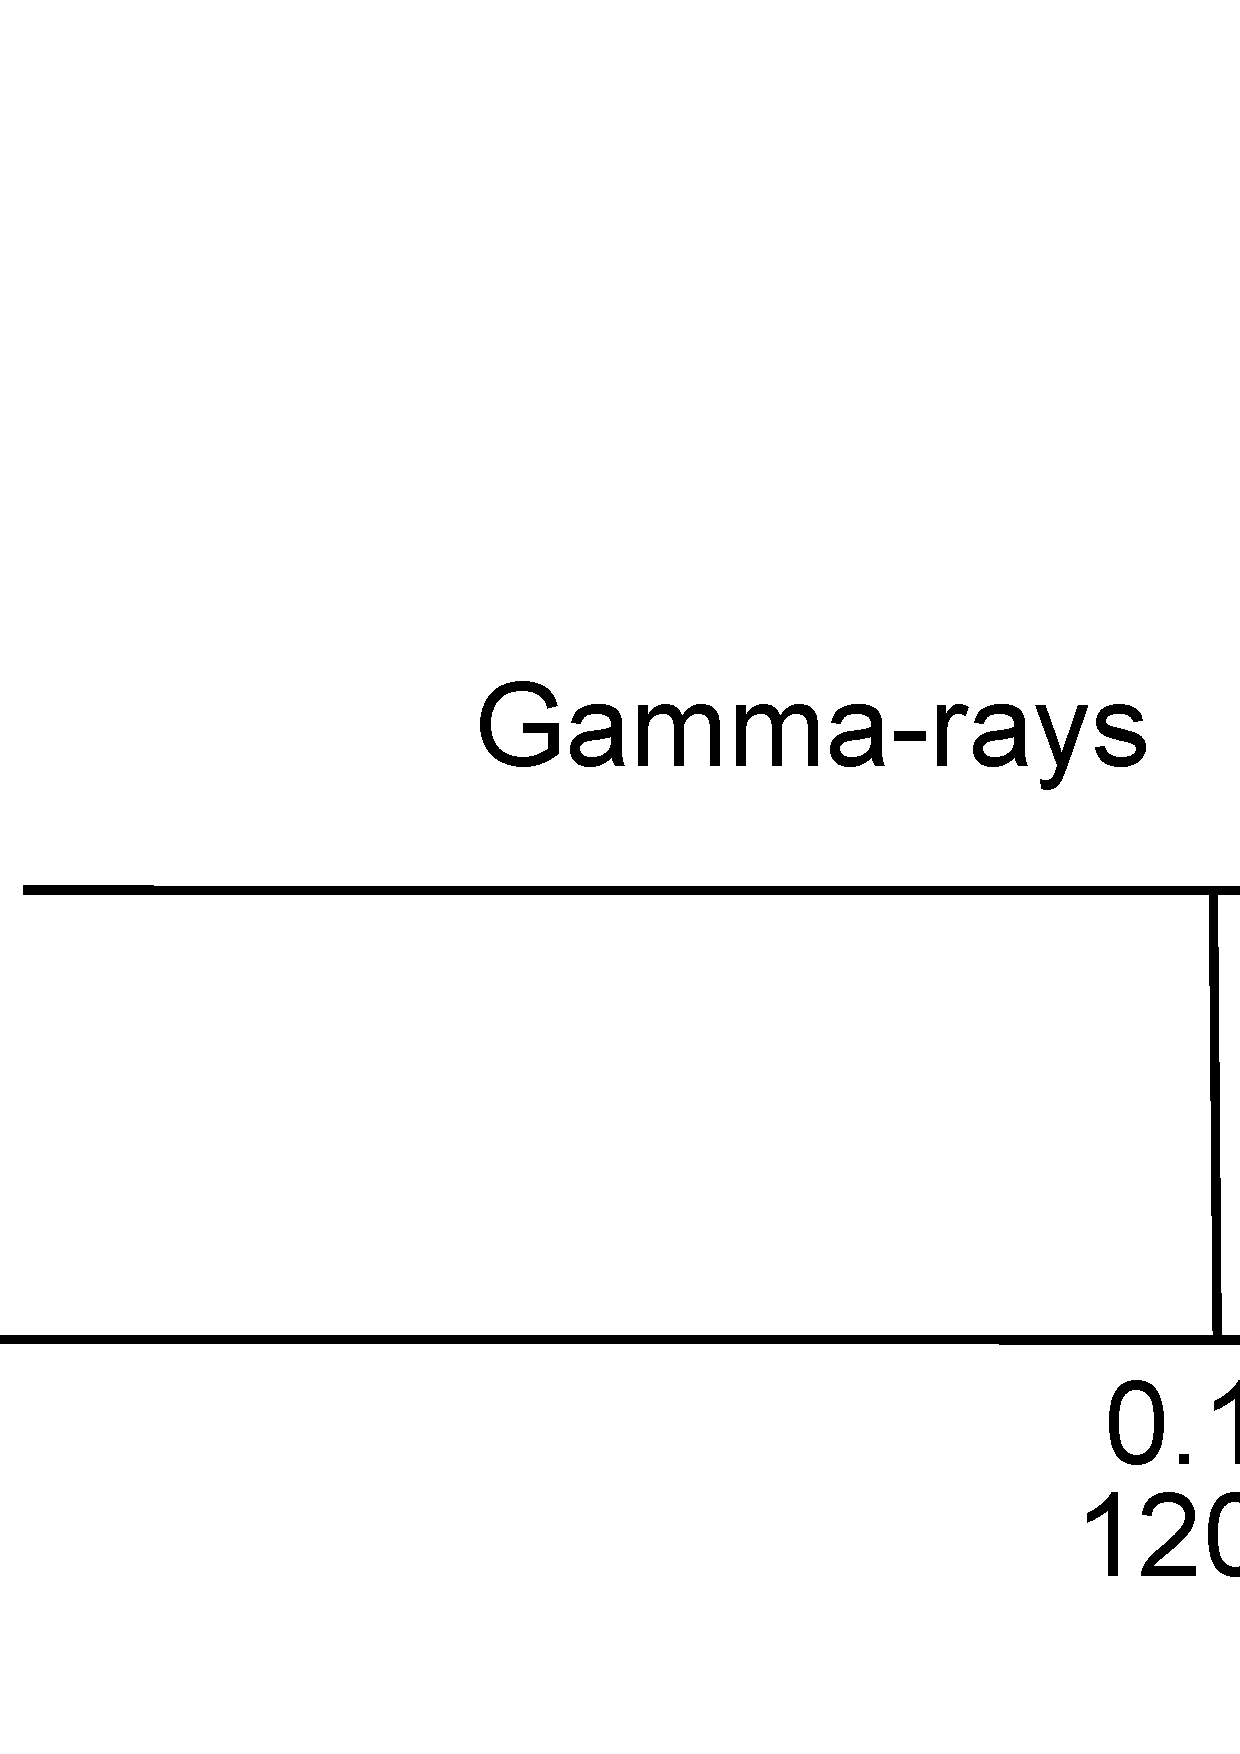
\includegraphics[width =\textwidth]{../introduction/images/spectrum.pdf}
\end{center}
\end{figure}
%
%One property of coherent X-emission is a phase relation between the spectral components of the pulse, which leads to short temporal duration (sub ps to fs) compared to incoherent X emission. Ultimately, fabrication of coherent X-ray sources lead to the study fondamental dynamics of matter such as the vibration of core electron wavefunctions in atoms and molecules or the motion of charged particles in solids or plasmas. 
%
%
%\begin{wrapfigure}
%\begin{center}
%\includegraphics[width =0.5\textwidth]{../introduction/images/Xfel-hamburg}
%\caption{Europeen XFEL facility, Hamburg (http://photon-science.desy.de)}
%\end{center}
%\end{wrapfigure}

\noindent Several conventional facilities can provide intense X-ray radiation. In case of synchrotrons, electrons are accelerated in km-long structures and their trajectories are modified with a combination of magnets (undulators) over a few meters. However, the coherence of such a source is limited and the emission does not go below a few picoseconds, mostly because of the electron bunch duration. Using a femtosecond laser to "slice" the electrons into short pulses, $\sim100\,\mathrm{fs}$ bursts were produced~\cite{schoenlein2000generation} on a synchrotron, but with a limited number of photons.
Free electron lasers (FEL)~\cite{madey1971stimulated,emma2010first,ribic2012status,corde2013femtosecond} are conventional accelerators which can produce intense X-rays~\cite{geloni2010coherence} with peak brightness\footnote{The peak brightness of an X-ray pulse is given in ph/s/0.1\%BW/mm$^2$/mrad$^2$~\cite{corde2013femtosecond}. It is different than the average brightness which accounts for the beam repetition rate} up to one million times greater than on synchrotrons, with pulse durations as short as $\sim 5\,\mathrm{fs}$~\cite{helml2014measuring}.  Although FELs are by far the most reliable installations to generate intense coherent X-rays, their size ($\sim  \,\mathrm{km}$ installations) and effective cost ($\sim G$euros) limit the number of users. In addition, sub-femtosecond X-rays pulses have so far never been achieved.\\

\noindent With the rapid increase of table-top laser peak powers ($> 10^{18}\,\mathrm{W/cm^2}$), it is possible to accelerate electrons in plasmas and generate X-rays. In 1977, Burnett and al. published the first experiment on the generation of X-UV radiation resulting from the interaction of a $\mathrm{CO}_2 $ laser with a plasma mirror~\cite{burnett1977harmonic} called high harmonic generation (HHG). The working principle is as follows: when an intense  laser pulse ($\sim 10^{15}\,\mathrm{W/cm^2}$)  reflects on a PM, electronic motion at the surface leads to the emission of coherent X-UV radiation with attosecond duration, every laser period. This produces a train of attosecond pulses seperated in time by one laser period. Therefore, these pulses interfere constructively in the spectral domain whenever the frequency is a multiple of the driving laser frequency, and for this reason are called high-order harmonics. However, the main limitation of these sources compared to conventional accelerators is the intensity of the source. It is also possible to perform HHG in gas jets with comparable generation efficiencies~\cite{sarukura1991coherent,macklin1993high,l1993high}, and generate X-UV pulses $<100\,\mathrm{as}$~\cite{zhao2012tailoring,goulielmakis2008single}. However, the laser intensity has to remain below the ionization threshold which is an intrinsic limitation of the possible brightness of the sources. On PMs however, the laser intensity can be in principle arbitrarily increased, simultaneously with the  brightness of the generated  X-ray sub-femtosecond bunches.\\

% records:
% FLASH: http://photon-science.desy.de/news__events/news__highlights/archive/archive_of_2006/world_record_at_flash/index_eng.html



%In the ``salle noire'' at LOA is located our sub TW , Ti-Sa laser system delivering a few mJ, $30\,\mathrm{fs}$ to 5$\,\mathrm{fs}$(current upgrade) pulses on target, which allows us to probe plasma dynamics looking at accelerate electrons and the generation X-UV harmonics of the driving laser at a repetition rate of 1kHz. 
% Every $\,\mathrm{ms}$, just before the arrival of the main pulse, the solid target has already turned into a plasma as the transition is fast with respect to the laser pulse ($\sim \,\mathrm{fs}$), but has no time to expand into vacuum (few ps) which makes it optically flat.  This PM is an ideal medium to perform extreme non linear interactions and in particular to generate X-UV coherent light or accelerate electrons and will be extensively disccussed in this manuscript.\\
%

\noindent Classically, a conversion efficiency is an non-dimensional quantity that measures an energy ratio $\eta = E_{out}/E_{in}$ associated with a given physical process. For high harmonic generation on PM, the efficiency is defined for a given frequency range so that $\eta (\omega)$ is an efficiency $/s^{-1}$. We write the energy conservation relation from the temporal to the Fourier domain (Parseval theorem): 

$$
\int_{\mathbb{R}}|E(\omega)|^2\frac{d\omega}{2\pi} = \int_{\mathbb{R}}|E(t)|^2 dt
$$

\noindent where $|E|^2$ is an energy density. Therefore, the energy contained in one attosecond pulse train is given by the harmonic conversion efficiency corresponding to the pulse spectral content. Based on numerical simulations, an integration of the laser energy before and after the interaction on target yields $75$\% reflectivity as presented in Fig~\ref{fig:spectraCamp}. A negligible fraction of the input energy is transfered to the harmonics. 

\begin{figure}[H]
\includegraphics[width =15cm]{../introduction/images/spectraCamp.pdf}\\
\caption{\label{fig:spectraCamp} Illustration of HHG for a 30fs laser pulse with intensity $ I = 10^{18}\,\mathrm{W/cm^2}$ on a PM with a density of 200$n_c$. The percentage of energy of the incident laser contained in the harmonics is given in yellow colors}
\end{figure}
% plasma gradient L/40

\noindent The harmonics shown in Fig~\ref{fig:spectraCamp} are generated with an exponentially decreasing conversion efficiency. This is typical of Coherent Wake Emission mechanism~\cite{Quere2006}, which we will describe in section~\ref{subsection:Plasma perturbative approach}. Here, the energy contained in the harmonics is expected to be linearly increasing with the laser intensity~\cite{plaja1998generation,thaury2010high}. At much higher intensity however, a new mechanism called Relativistic Oscillating Mirror~\cite{Thaury2007} is now responsible for the emission. For this mechanism, it has been predicted that an increase of the laser intensity would simultaneously enhance the generation efficiency~\cite{thaury2010high}. Numerical simulations performed with a laser intensity of $\sim 10^{19}\,\mathrm{W/cm^2}$ indicate that sub-fs X-UV emission can reach several percent~\cite{Naumova2004} (mostly contained in low HHG orders) and therefore compete with peak-brightnesses obtained using X-FEL lasers.


 \subsection{Electron acceleration from plasma mirrors}

 High energy particle radiation started to become an attractive source for various application after the discovery of artificial nuclear reactions between 1910 and 1930. Physicists had access to alpha and beta particles resulting from nuclear reaction products~\cite{rutherford1916xliii}, but were limited in energy and flux. 
 In 1927, Rutherford, publicly announced at the Royal Society of London his ``\textit{ambition to have available for study a copious supply of atoms and electrons which have an individual energy far transcending that of the alpha and beta particles}”. 
 In 1929, Walton and Cockcroft built the first proton accelerator to perform fundamental nuclear experiments by means of a high-voltage static electric field $\sim 10^6\,\mathrm{V}$, accelerating protons up to $300\,\mathrm{keV}$~\cite{cockcroft1930experiments,cockcroft1932experiments}. This was sufficient to manage the transmutation of lithium nuclei, for which they received a Nobel Prize in 1951. Another type of electrostatic accelerator, developed in parallel by Van de Graff consisted in transporting charges in a moving belt, lead to particles accelerated up to $\sim 15\,\mathrm{MeV}$. During the same period, a new type of accelerator invented by Lawrence in 1932, called cyclotron, was born. The principle is to use a magnetic field to confine electrons into a spiral while a radio-frequency electric field $\sim 10^3\,\mathrm{V}$ accelerates them (or other charged particles). 
  After World War II, a variant of cyclotrons called ``synchrotrons'', still widely used today in medical applications, was born. Because the research had been so far mostly driven by nuclear research, most experiments consisted in the acceleration of charged ions. However, electrons which are also charged and almost two thousand times lighter that protons can also be accelerated, and their trajectories are easy to modulate in time. The first electron accelerator principle was proposed by D. W. Kerst in 1940 and was based on betatron acceleration (synchrotron for ``beta'' particles)~\cite{kerst1940acceleration} followed by successful table-top proof-of-principle at the University of Illinois. In 1945, $100\,\mathrm{MeV}$ electrons were accelerated at General Electric based on this principle. Betatron accelerators were for instance used in the Manhattan project to investigate some basic radioactive components properties. Electrons are accelerated in a circular vacuum chamber through an inductive effect: an alternative magnetic field generates an accelerating radial electric field. Note that a betatron and a linear induction accelerator are quite similar with the difference that the trajectories are circular in case of betatrons. In fact, for acceleration to be significant, electrons need to be circulated millions of times in the toroidal chamber, which explains why an additional magnetic field is added to prevent them from escaping their circular orbits of radius $R$.


\begin{equation}
E(\mathrm{MeV}) \le 300 B_s(\mathrm{T}) R(\mathrm{m})
\end{equation}

\noindent For example, an energy of $450\,\mathrm{MeV}$ could be reached theoretically taking $R = 1\,\mathrm{m}$ and $B_{s} = 1.5\,\mathrm{T}$. Betatrons are limited in terms of acceleration because of the finite magnet size and radiation losses of the charged particles, but they have the great advantage of being compact devices, which makes them very appealing for industrial and medical applications.\\

\noindent But since the 80's, laser-driven plasma acceleration techniques have emerged: intense laser pulses focused into a gas jet generates compact accelerating structures where the electric field reaches $\sim $TV/m. The concept of plasma acceleration was introduced by Dawson and Tajima in 1979~\cite{tajima1979laser}. The idea is to focus a beam into a gas jet to generate a micrometer accelerating cavity called wakefield. A wakefield cavity resembles that of a RF linear accelerator, but electric fields are orders of magnitude higher. The use of an energetic electron or ion beam was suggested in 1994 to trigger the fusion reaction of laser compressed deuterium pellets~\cite{tabak1994ignition}. In this so called "fast ignition" scheme, $\sim 1\,\mathrm{MeV}$ suprathermal electrons are produced in the interaction of an intense laser at the surface of the compressed pellets, which propagate towards the core where they deposit their energy. This mechanim, fully supported by simulations~\cite{tabak1994ignition} has not yet been demonstrated experimentally. This initially explained the growing interest of the community in laser-driven solid-density experiments~\cite{honrubia2006three,Brunel1987,Gibbon1992,askar1994magnetic,pukhov1996relativistic,sheng2002stochastic}. In Chapter~\ref{Anticorrelated harmonic and electron emission from plasma mirrors}, we will give a more detailed description of the different mechanisms involved in the interaction of an intense laser beam with a solid density plasma, leading to electron acceleration. \\

\noindent However, as we already mentioned, a solid density plasma is not necessarily a plasma mirror. When the plasma expands into vacuum, its surface quality degrades and the laser interacts with the underdense region of the plasma before it is reflected as described in chapter~\ref{chapter:Laser-solid-plasma interaction: overview}. Few experiments have so far been conducted on the acceleration of electrons from plasma mirrors~\cite{mordovanakis2009quasimonoenergetic,thevenet2015}. The work presented in this PhD focuses on the exploration of this interaction in the sub-relativistic regime. In particular, we will describe the prerequisites for efficiently accelerating electrons from plasma mirrors.



%
%When a laser pulse propagating in vacuum interacts with matter, the electromagnetic energy it carries can either be reflected, transmitted or absorbed. 
%Those three responses usually occur simultaneously and previledge absorption, reflection or transmission will depend on the laser caracteristics (frequency, pulse duration, intensity ..) and on the medium chosen for the interaction (gas,dielectric, metal, plasmas..) as well as the nature of the vacuum/matter interface (polished, plane, periodically structured..). If we consider a solid for the interaction (typical density of $\sim 10^{23}\,\mathrm{atoms/cm^3}$), it is well known that if the laser frequency matches the electron bounding energies of the atoms, the solid is ionized. 
%The study of laser/plasma interactions is more the 50 years old, and laser absorption have often been attributted to collisions between charged particles, which means transforming coherent electromagnetic radiation into thermal energy (joule effect). But up untill the emmergence of mode-locked femtosecond lasers, the typical time scale on which plasmas were investigated was limited to the nansecond (CO2 lasers for instance) and later to the picosecond (Q-switch) timescale which is much greater than the caracterisic time known for collisions ($\sim $ fs). 






\newpage




\section{Brief description of the different chapters}

\begin{itemize}
\item[$\bullet$]  \g{Chapter~\ref{chapter:Laser-solid-plasma interaction: overview} :} In this chapter, we describe the basic mechanism behind laser absorption on thin plasma mirrors. We present in detail the so-called "resonant absorption" mechanism, as well as "Brunel Absorption" mechanism, better suited for plasmas with very short scale lengths. In a second time, we will see how a dense plasma responds to an electronic perturbation by generating X-UV light, and discuss the asymptotic case of very long and very short plasma scale length, where this emission can no longer take place. 

\item[$\bullet$]  \g{Chapter~\ref{chapter:Overall presentation of the laser system}}: In this chapter, we describe the global architecture of our laser. After a brief presentation of the main components, we focus on XPW contrast cleaning and present a source of temporal contrast degradation in our CPA. After discussion on the laser contrast and the possible way of improving it, we describe the solid-target interaction chamber. In particular, we will present the $1 \mathrm{kHz}$ rotating target and the main beam characteristics (spatial, temporal) on target.


\item[$\bullet$]  \g{Chapter~\ref{chapter:Properties of attosecond pulses emitted using plasma mirrors}}: In this chapter, we will recall some of the basic properties of Coherent Wake Emission (CWE). The reader is invited to check the provided references for a more detailed description. In a second part, we will see how the divergence and spectral properties of the emitted harmonics are sensitive to spatio-temporal couplings (STC) of the driving laser. In particular, we will show how it is possible to experimentally control an STC of first order called Wave Front Rotation (WFR) and how it can affect harmonic generation. This technique has been already tested successfully to seperate attosecond pulses from plasma mirror by changing over time their direction of emission~\cite{Wheeler2012}. Here we discuss the possibility of retrieving temporal information on the attosecond train when the pulses are not separated.  


\item[$\bullet$] \g{Chapter~\ref{ch:Measuring the gradient expansion}}: In this chapter we present a technique developed during this PhD called spatial domain interferometry (SDI), which allows us  to measure the expansion velocity of the plasma generated on the solid target by a controlled prepulse. We will then discuss the current limitations of this technique such as the pointing stability of the pulses on target, and how it can be easily identified using the intensity profile of the reflected probe. Finally, we will suggest to go one step further with the implementation of a phase-retrieval algorithm allowing the two-dimensional reconstruction of the plasma during its expansion.


\item[$\bullet$]  \g{Chapter~\ref{Anticorrelated harmonic and electron emission from plasma mirrors}}: In this chapter, we present experimental results of the simultaneous observation of harmonics and electrons from plasma mirrors. In particular, we show how the emission is anticorrelated with the gradient scale length. We then present the measured electron angular emission profile and energy spectra depending on the plasma scale length.




\item[$\bullet$]  \g{Chapter~\ref{Laser-electron interaction in vacumm}}: This chapter focuses on electron interaction with the laser when it reflects on the plasma surface. We discuss two different regimes namely ``ponderomotive'' and ``non ponderomotive'' laser acceleration in vacuum, and in particular how they depend upon the laser intensity. We also discuss the effect of our strong focusing geometry  on the angular emission profile of electrons.

\end{itemize}



































